First we developed a new, unified framework for implementing turnover. 
We then simulated a deterministic, compartmental model of
an illustrative STI to carry out the experiments.

% SM: consistency & double-checks
% modelliing vs. modeling
% avoid using the words 'this', 'these', etc. as much as possible. Used **a lot** throughout methdods section reviewed so far
%SM: consistency check with numbers (3 or three)
% ==================================================================================================
\subsection{A unified framework for implementing turnover} %we do not use the term 'turnover system' before, so even though more words - would suggest we try to use same phrasing throughout. we introduce a lot of new terminology in the paper, and so the fewer new 'terms/phrases' that need to be defined --> the eaiser it will be for the reader
%     (PS not addressing other comments yet in this edit)
\label{ss:system}
\begin{figure}
  \centering
  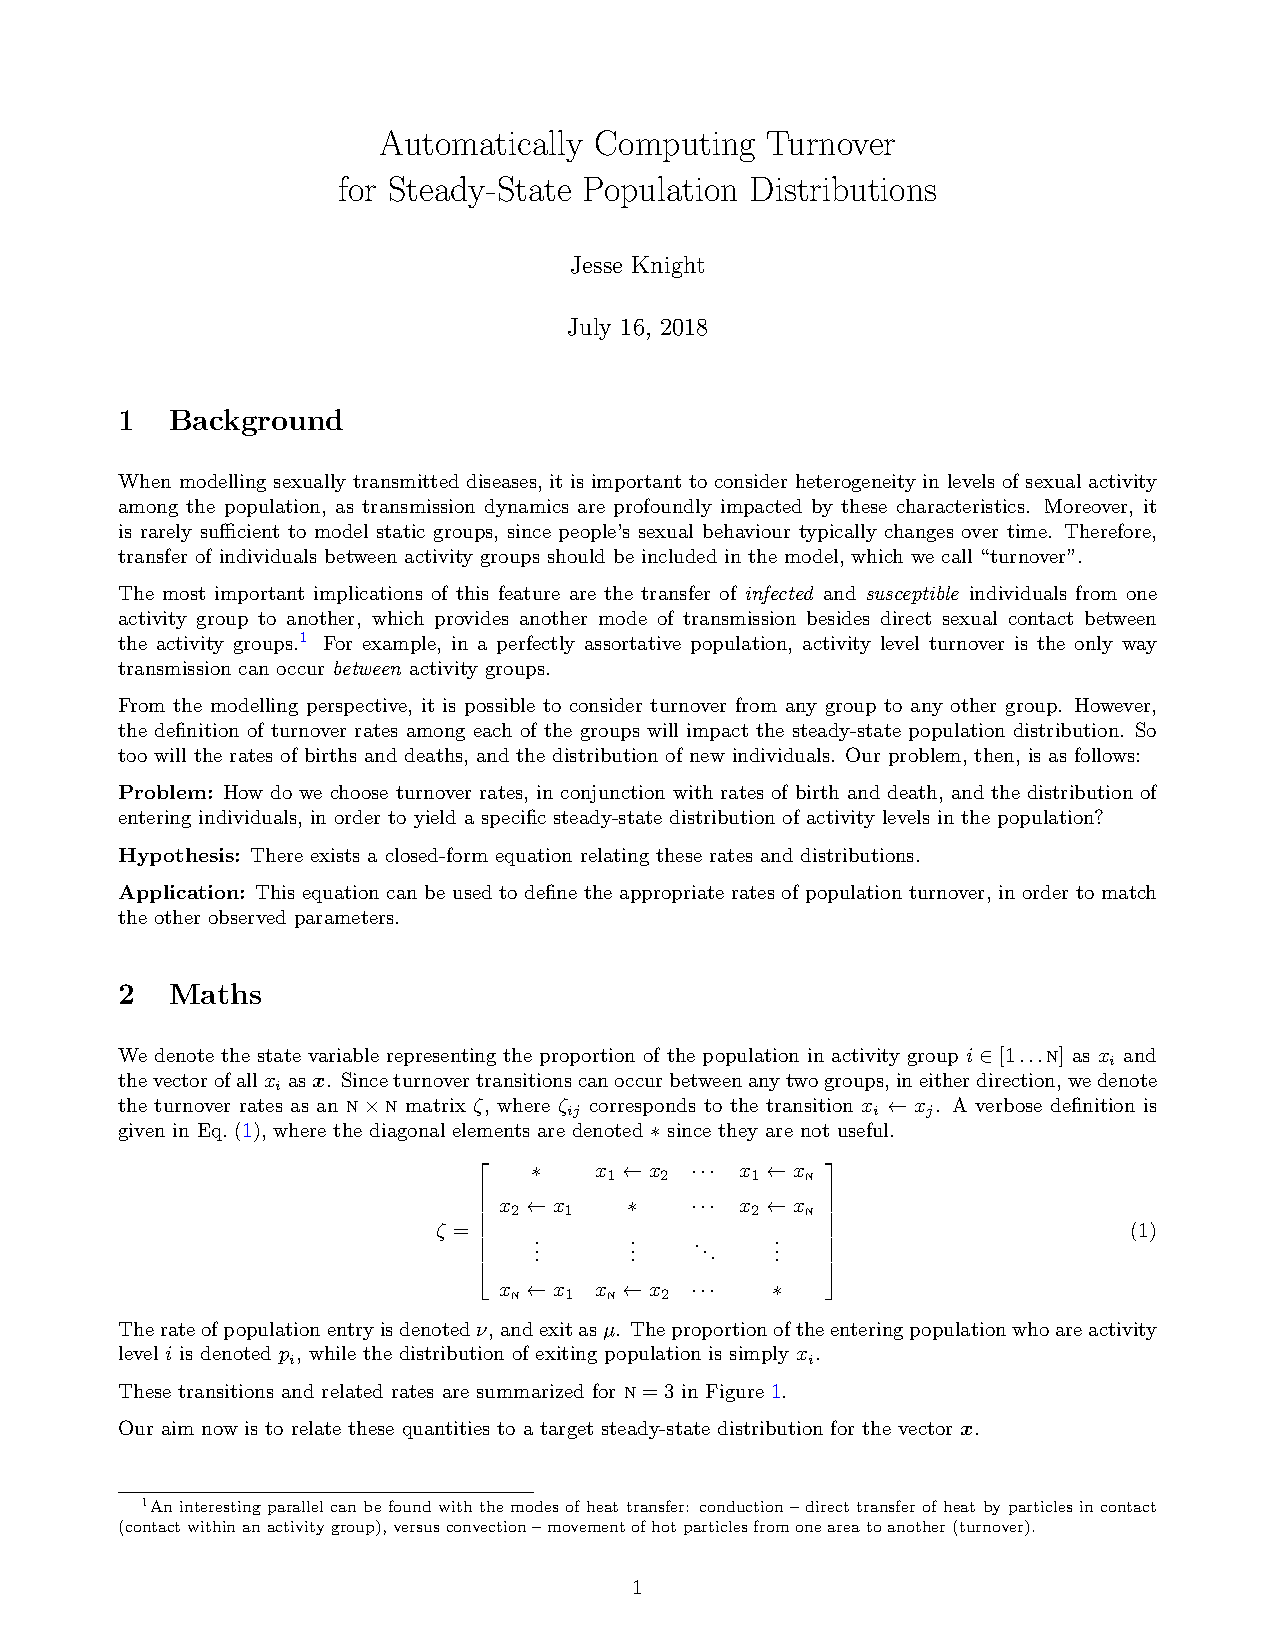
\includegraphics[width=0.5\linewidth]{turnover}
  \caption{System of risk groups and flows between them for $G = 3$}
  \label{fig:system}
\end{figure}
We developed a framework for implementing turnover,	
as depicted in  Figure~\ref{fig:system}.
and detailed in the Appendix~\ref{a:system}. 
In the framework, the simulated population is divided into $G$ risk groups.
The number of individuals in group $i \in [1, \dots, G]$ is denoted $x_i$,
and the relative size of each group is denoted $\hat{x}_i = x_i / N$,
where $N$ is the total population size.
Individuals enter the population at a rate $\nu$ and exit at a rate $\mu$ per year.
The distribution of risk groups at entry into the model
is denoted $\hat{e}_i$, which may be different from $\hat{x}_i$.
The total number of individuals entering group $i$ per year
is therefore given by $\nu \hat{e}_i N$.
Turnover rates are collected in a $G \times G$ matrix $\phi$,
where $\phi_{ij}$ is the proportion of individuals in group $i$
who move from group $i$ into group $j$ each year.

The framework only considers demographic transitions between risk groups, and does not
include any health-states. That is, we assume that rates of turnover $\phi$
do not vary by the health state of individuals. 		%But health-states have not been described yet. Seems funny to write it into the unified system noh? Perhaps should say that the unified system is independent of the disease model, and thus, independent of the health-states, or something like that?
\par
For our specific research questions,			%Clarify that the 'we assume' part is specific to the research question - i.e. for the set of experiments in the current paper. vs. the unified framework assumes that the relative size of risk groups remain stable, etc. 
we assumed that the following: (1) the relative sizes of risk groups		%consider list/number the assumptions to help the reader navigate and follow the thought process	
$\bm{\hat{x}} = [\hat{x}_1, \dots, \hat{x}_G]$
are known and should remain constant over time; and (2) 
the rates of population entry $\nu$ and exit $\mu$
are known, but that they may vary over time.
The approach to estimate $\nu$ and $\mu$ is detailed in Appendix~\ref{aaa:params-nu-mu}.
Thus, what remained was to estimate $\bm{\hat{e}}$ and $\phi$,
representing $G + G(G-1) = G^2$ unknown values.

In the framework,
the parameters (%SM: list parameters) 
are collected in the vector   %change variable to parameter. 'variables' have a very specific meaning in ID modeling (state variable and force of infection terms). What does 'these parameters' refer to? 
$\bm{\theta} = \left[\bm{\hat{e}}, \bm{y}\right]$,
where $\bm{y} = \mathrm{vec}_{i \ne j}(\phi)$.
To uniquely determine the elements of $\bm{\theta}$, we
we constructed a set of linear constraints.
Each constraint $k$ took the form		%SM: remove 'this' and 'these' from every sentence in paper, and then put back in with a clear definition of the subject :) 
$b_k = A_k \bm{\theta}$,
% JK: present tense for notation
where $b_k$ is a constant and $A_k$ is a vector with the same length as $\bm{\theta}$.
The values of $\bm{\theta}$ were then obtained by solving
%\begin{equation}\label{eq:system-matrix}
$\bm{\theta} = A^{-1}\bm{b}$,
%\end{equation}
using existing algorithms~\citep{LAPACK}. %SM: specify what type of algorithm: eg. optimization algorithms for soliving linear systems? 
\par
The framework defines four types of constraints which can used to
solve for the values of $\bm{\hat{e}}$ and $\phi$ via $\bm{\theta}$.
The frameworks supports flexibility with respect to selecting and combining
constraints, guided by data availability and the underlying assumptions.
However, a minimum of $G^2$ non-redundant constraints had to be specified
to produce a unique solution such that one value of $\bm{\theta}$ satisfies all constraints. %SM: using -- word -- is for emphasis in place of commas usually. don't think aposthrophes needed.
Table~\ref{tab:constraints} summarizes 
the four types of constraints, with their underlying assumptions and the type of data which
can be used to inform the parameters.									%SM: the term 'define' takes on various meanings in the text. review for consistency.
Additional details, including
constraint equations, examples, and considerations for combining constraints,
are in Appendix~\ref{aaa:params-turnover}.%							%SM: hard copy of edits on your desk. the references need some work.
\begin{table}
  \centering
  \caption{Summary of constraint types for defining risk group turnover}
  \label{tab:constraints}
  \begin{tabular}{clccl}
	\toprule
	   & Name                       &            Eq.            &        E.g.         & Data requirements                                                         \\
	\midrule
	1. & Constant group size        & (\ref{eq:mass-balance-2}) & (\ref{eq:eg-basis}) & all values of $\hat{x}_i$ and $\nu$                                       \\
	2. & Specified elements         &   (\ref{eq:spec-elem})    & (\ref{eq:eg-spec})  & any value of $\hat{e}_i$ or $\phi_{ij}$                                   \\
	3. & Group duration             & (\ref{eq:duration-group}) &  (\ref{eq:eg-dur})  & any value of $\delta_i$                                                   \\
	4. & Relative rates of turnover &     (\ref{eq:ratio})      & (\ref{eq:eg-ratio}) & any relationship between two turnover rates $\phi_{ij}$ and $\phi_{i'j'}$ \\
	\bottomrule
\end{tabular}\\[1em]
\footnotesize\flushleft
$\nu$:~rate of population entry;
$\phi_{ij}$:~rate of turnover from group $i$ to group $j$;
$\hat{x}_i$:~proportion of individuals in risk group $i$;
$\hat{e}_i$:~proportion of individuals entering into risk group $i$;
$\delta_i$:~average duration spent in risk group $i$.
\end{table}
% ==================================================================================================
\subsection{Transmission model}\label{ss:model-sim}						%can you point to the Appendix where the ODEs for the transmission model can be found?
We developed a deterministic, compartmental model of an illustrative 
sexually tranmitted infection with 3 risk groups. We did not
simulate a specific pathogen, but rather selected a biological system
that included susceptible, infectious, and treated (or recovered/immune) health-states. 
The transmission model thereofore was mechannistically representative of sexually transmitted infections like
HIV (where effective antiretroviral treatment reflects a health-state where individuals
are no longer susceptible nor infectious) or hepatitis B virus (where among the large proportion
of individuals who clear their acute infection, develop life-long protective immunity). %SM: find a citation for the natural history of HBV infection (e.g. a major review paper)

The model is represented by a set of coupled, ordinary differential equations (shown in AppendixXX) and
includes three health states:
susceptible~$\mathcal{S}$, infectious~$\mathcal{I}$, and treated~$\mathcal{T}$
(Figure~\ref{fig:health-states}),
and $G = 3$ levels of risk:
high~$H$, medium~$M$, and low~$L$.
\begin{figure}
  \centering
  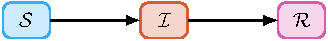
\includegraphics[width=0.4\linewidth]{health-states}
  \caption{Modelled health states.
    $\mathcal{S}$: susceptible;
    $\mathcal{I}$: infected;
    $\mathcal{T}$: treated;
    $\lambda$: force of infection;
    $\tau$: treatment.}
  \label{fig:health-states}
\end{figure}
Risk strata were defined by different number of contacts per year
so that individuals in risk group $i$ were assumed to
form contacts at a rate $C_{i}$ per year.
The probability of contact formation $\rho_{ik}$ between individuals in group $i$
and individuals in risk group $k$ was assumed to be
proportionate to the total number of available contacts within each group:
\begin{equation}
\rho_{ik} = \frac
{C_k x_k}
{\sum_{\mathrm{k}}C_{\mathrm{k}} x_{\mathrm{k}}}
\label{eq:rho}
\end{equation}
\par
The biological probability of transmission was defined as $\beta$ per contact.
Individuals transitioned from the
susceptible $\mathcal{S}$ to infectious $\mathcal{I}$ health-state
via a force of infection $\lambda$ per year, per susceptible in risk group $i$:
\begin{equation}
\lambda_{i} =
C_{i} \sum_k \rho_{ik} \thinspace  \beta \thinspace \frac{\mathcal{I}_k}{x_k}
\label{eq:foi}
\end{equation}
Individuals were assumed to transition from the
infectious $\mathcal{I}$ to treated $\mathcal{T}$ health-state
at a rate $\tau$ per year, reflecting diagnosis and treatment.
The treatment rate did not vary by risk group.
Individuals in the treated $\mathcal{T}$ health-state were neither infectious nor susceptible,
and individuals could not become re-infected.
% --------------------------------------------------------------------------------------------------
\subsubsection{Implementing turnover within the transmission model}
As described in Section~\ref{ss:system}, individuals
entered the model at a rate $\nu$,
exited the model at a rate $\mu$,
and transitioned from risk group $i$ to group $j$ at a rate $\phi_{ij}$.
The turnover rates $\phi$ and
distribution of individuals entering the model by risk group $\bm{\hat{e}}$
were computed using the methods outlined in
Appendix~\ref{aaa:params-turnover}, based on the following three assumptions.			%SM; assumption, or condition, or constraint? 
% SB: Do we need to explain why we made these assumptions? Or provide refs?
% JK: Since we are constructing a simulated system, I'm not sure what refs might be appropriate,
%     but, you make a great point about justifying.
%     I've added a sentence after all 3 assumptions explaining.
%     I think I was avoiding this because it was hard to explain,
%     but let me know how it reads.
First, we assumed that
the proportion of individuals entering each risk group $\bm{\hat{e}}$
was equal to the proportion of individuals across risk groups in the model $\bm{\hat{x}}$.
% LW: And another strong assumption which was implicit here is that u assume
%     the rate of turn over to be the same irrespective of disease status.
%     And I think it is critical to make it explicit.
%     So S, I, T all have the same turn over rate,
% JK: So, I did now include this in the Turnover System section (last sentence).
%     Do you think it needs to be restated here? SM: yes, re-iterate here (before 'first')
Second, we assumed that
the average duration spent in each risk group $\bm{\delta}$ was known.
Third, we assumed that
the absolute number of individuals moving between two risk groups in either direction was balanced such that
the proportion of individuals in each risk group remain stable over time.   %SM: yes agree a strong assumption, but one that most models make. So make sure to discuss each of these 
%excellent points by SB and LW and HM in the discussion!
% LW: I would think this is a very strong assumption.
%     It is essentially saying the turn-over system consistently
%     *swap* individuals in two risk groups.
% HM: Not fully understand how does this assumption work?
%     If high risk group has 10 individuals move to medium group,
%     medium group will move 10 individuals to high risk? This is independent from population entry?
% JK: @HM: yes, this is what this assumption means. I've edited hopefully to be more clear.  %SM: could be more clear. suggest giving an example  as HM did in her comments.
%     @LW: see new sentence below. We have to make at least one more assumption,
%     else the system will not have a unique solution,
%     and by "balancing" the turnover rates, it is a way of avoiding "bias":
The above assumptions, and therefore constraints, were selected
because they reflect the common assumptions underlying turnover in prior models	%SM: cite (as per introduction)
and also to avoid any dominant direction of turnover. That is, 
we wanted to restrict our analyses to the influence of movement
between risk groups in general (compared with no movement and at
various overall rates of movement) rather than 
unidirectional movement from one just one group to another.
The system of equations formulated from the above assumptions and constraints
is given in Appendix~\ref{aa:eqs-turnover}.

To meet all three conditions, there was only one possible value			%what do you mean by 'condition' here? constraints? 
for each element in $\phi$ and $\bm{\hat{e}}$.
That is, by specifying the three conditions,						%it gets frustrating for the reader to see various terms like this!
we were able to generate a unique set of $\phi$ and $\bm{\hat{e}}$.		%try for more active voice 
\par %SM: I did not understand the paragraph below. 
Using the above three assumptions,							%conditions or assumpiton? ugh.... starting to frustrate the reader dude! :) 
we needed to specify the values of $\bm{\hat{x}}$, $\bm{\delta}$, $\nu$, and $\mu$.
Such parameters could be derived from data as described in Appendix~\ref{aaa:params-turnover}.
However, in this experiment, we used the illustrative values summarized in %SM: what does 'this' refer to? which experiment? the whole study? there are 3 experiments noh? poor  reader is wanting to give up soon :) !
Table~\ref{tab:params}.
% LW: After read the whole results section,
%     I think experiment 2 and 3.2 followed values specified in Table 3.
%     But experiment 1 and 3.1 explored a wide range of
%     turn-over and treatment rates.
%     it is unclear what do u refer to when u said “this experiment”.
%     Given the organization and length – by the time I reached results of Experiemnt 2,
%     I almost forgot under which values they were done – as the section preceed it
%     explored a range of values of turn-over rate and treatment rate.
% JK: Hopefully now with the paper much much shorter, this is resolved?
After resolving the system of equations,
$\bm{\hat{e}}$ was equal to $\bm{\hat{x}}$ (assumed), and $\phi$ was:
\begin{equation}
\label{eq:phi-values}
\phi = \left[\begin{array}{ccc}
* & 0.0833 & 0.0867\\
0.0208 & * & 0.0158\\
0.0058 & 0.0042 & *
\end{array}\right]

\end{equation}
\begin{table}
  \centering
  \caption{Model parameters}
  \label{tab:params}
  \begin{tabular}{clc}
	\toprule
	    Symbol     & Description                                                     &            Value             \\
	\midrule
	 $\bm{\beta}$  & transmission probability per contact                            &            $0.03$            \\
	    $\tau$     & rate of treatment initiation among infected                     &            $0.1$             \\
	    $N_0$      & initial population size                                         &            $1000$            \\
	\midrule
	$\bm{\hat{x}}$ & proportion of system individuals by risk group                  & $[ 0.05 \es 0.20 \es 0.75 ]$ \\
	$\bm{\hat{e}}$ & proportion of entering individuals risk by risk group           & $[ 0.05 \es 0.20 \es 0.75 ]$ \\
	$\bm{\delta}$  & average duration spent in each risk group                       &    $[ 5 \es 15 \es 25 ]$     \\
	     $C$       & rate of contact formation among individuals in each risk group  &     $[ 25 \es 5 \es 1 ]$     \\
	    $\nu$      & rate of population entry                                        &            $0.05$            \\
	    $\mu$      & rate of population exit                                         &            $0.03$            \\
	\bottomrule
\end{tabular}
  % SS: All of this seems a little hard to follow in terms of the infection,
  %     b/c it seems to indicate that there is an underlying infection of interest,
  %     but it is not being stated.
  % JK: Same as above, not sure what to say here...
  %     We did start out with HIV, but since we're not considering STI-mortality,
  %     we really cannoy call it HIV.
\end{table}
\par
We then simulated epidemics using the parameters %SM: list the parameters or say in $\phi$ .
The transmission model was initialized with $N_0 = 1000$ individuals
who were distributed across risk groups according to $\bm{\hat{x}}$.
We seeded the epidemic with
one infectious individual in each risk group at $t = 0$ in an otherwise 
fully susceptible populatuon.
We numerically solved the system of ordinary differential equations			%SM: did you tell the reader where the ODEs are, in description above?
in Python%
\footnote{Code for all aspects of the project is available at:
  \href{https://github.com/c-uhs/turnover}{\texttt{https://github.com/c-uhs/turnover}}}
using Euler's method with a time step of $dt = 0.1$ years.
The set of coupled ordinary differential equations is in Appendix~\ref{aa:eqs-model}.		%SM: should be in the section on the transmission model I think

% ==================================================================================================
\subsection{Experiments}
\label{ss:exp}
We designed three experiments to examine the influence of turnover.
We compared outcomes at equilibrium,
defined as a steady state at 500 years with $<1\%$ difference in incidence per year.

% --------------------------------------------------------------------------------------------------
\subsubsection{Experiment~1: Influence of turnover on equilibrium incidence and prevalence}
\label{sss:exp-prev-inc}
We designed experiment~1 to explore the mechanism by which turnover influences
the equilibrium incidence and prevalence of infection, and the ratio of prevalence between risk groups (prevalence ratios).		%SM: make sure the order of incidence/prevalence is consistent througout paper. i think based on the results, you start with prevalence and then incidence. so order that way in writing throughout the methods. Introduce the outcome = prevalence ratios up front here.
We defined incidence as $\lambda_i$ from Eq.~(\ref{eq:foi}), and
prevalence as $\hat{\mathcal{I}}_i = \dfrac{\mathcal{I}_i}{\mathcal{X}_i}$.
% SM: start by something like this to orient the reader
%     and help with interpretation before results section
% JK: I agree this could be useful, but then we go back-and forth between
%     implementation ("controlled by a single parameter") and
%     an overview of the experiment ("influence of turnover on ...")
%     I'd rather introduce how turnover is controlled via duration in high risk group
%     after noting why we cannot simply scale the rates proportionally with a single parameter. %SM: I found it easy to follow the current version.
Similar to previous studies, \citep{Zhang2012,Henry2015},		%SM: because already mentioned the two studies in the introduction, I think do not have to go into detail here that the two studies examined influence of turnover on other modeled outcomes, etc.
we scaled (varied) the rates of turnover using a single parameter.

However, because our model had $G = 3$ risk groups,
multiplying a set of base rates $\phi$ by a scalar factor
would change the relative population size of risk groups $\bm{\hat{x}}$. 	%SM: consistency check: relative population sizes vs. sizes vs. size ... of risk groups
Thus, to explore the influence over a range of turnover rates 
but keep the relative size of each risk group stable, we 
controlled the rates of turnover using
the duration of individuals in the high risk group $\delta_H$.
We used the duration of time spent in the high risk group as the mediator of overall turnover
because of its practical interpreation in the context of STI transmission:
the duration in formal sex work for example.						%cite: Watts
A shorter $\delta_H$ implied higher rates of turnover among all groups.		%implied or means or is equivalent to? 'implied' seems vague?
The duration of time spent in the medium risk group $\delta_M$			%SM: duration of individuals reads funny. please change throughout. duration of time. duration of person-years. but people do not have durations so grammatically sounds really odd.
was then defined as a value between $\delta_H$ and the maximum duration $\mu^{-1}$
which scaled with $\delta_H$ following:
$\delta_M = \delta_H + \kappa \left(\mu^{-1} - \delta_H\right)$, with $\kappa = 0.3$.
The duration of time in the low risk group $\delta_L$
similarly scaled with $\delta_H$,
but due to existing constraints,
specification of $\delta_H$ and $\delta_M$
ensured only one possible value of $\delta_L$.
Thus, each value of $\delta_H$ represented a unique set of turnover rates $\phi$
whose elements all scaled inversely with the duration in the high risk group $\delta_H$.
					The duration of time spent in each group as function of the turnover in the high risk group 
is shown in Figure~\ref{fig:dur-group}.
\begin{figure}
  \centering\includegraphics[width=0.45\linewidth]{{1d-dur-all-tau=0.1}.pdf}
  \caption{Average duration in each risk group as turnover rates vary.}
  \label{fig:dur-group}
\end{figure}
\par
We then compared the equilibrium prevalence (in each risk group and in the
total population) across the range of $\delta_H$ = 33~to~3 years.						%SM: justify why chose 33 to 3 years. We selected the range to reflect reports of average duration in sex work as short as 2-3 years (%cite) and the average life-span in the model of 33 years, which generally reflects the average duration of sexual activity (age 14-X years) commonly assumed in STI transmssion models. % cite (e.g. Garnett review/explanatory paper on STI modeling and vaccines I think?)
To explain the observed relationships, we.... %SM: ??did what? 
% --------------------------------------------------------------------------------------------------
\subsubsection{Experiment~2: Inferred risk heterogeneity with vs without turnover}
\label{sss:exp-infer}
We designed experiement~2 to examine how the inclusion of turnover
(vs. absence of turnover) could change inference on other transmission model parameters 
related to risk heterogeneity: specifically,
the ratio of partner numbers  $C$ across risk groups.							%SM: call it partnership rates. in the discussion, can go into how findings could be generalized to contacts. but you balanced partnerships so partner numbers is easier to follow.
The ratio of partner numbers $C_H~/~C_L$
is one way to measure of how different the two 
risk groups are with respect to their 
acquistion and transmission risks.	 
Indeed, ratios of partner numbers are often used when parameterizing 
risk heterogeneity in STI transmission models.						%SM: cite. General principle throughout - justify or give rationale for the choices and selections always. Cannot emphasize enough in modeling (and all science actually) re: good practice! :) 
				
First, we independently fit the transmission model with turnover 
and without turnover, to
equilibium infection prevalence across risk groups. Specifically, we 
held all other parameters at their default values and
fit the partner numbers $C$ in each risk group	to reproduce the following:
20\% infection prevalence among the high risk group,
8.75\% among the medium risk group,
3\% among the low risk group,
and 5\% overall.
To identify the set of paramters (i.e.  partner numbers $C$ in each risk group)
that best reproduced the fitting targets, we minimized
the negative log-likelihood of group-specific and overall prevalence.%				%SM: most journals do not like footnotes. Check if Epidemics allows. I believe IDM does not. Journals like AJE, IJE, Lancet, JAIDS, etc. do not allow footnotes except in tables. So you may need to move to the methods or put into appendix.
\footnote{Sample sizes of 500, 2000, 7500, and 10,000 were assumed to generate binomial distributions
  for the high, medium, low, and overall prevalence targets respectively,				%SM: justify the use of these sample size as sample size would effect the log-liklihood term. For example, did you choose them based on typical surveys of such groups when prevalence is measured? e.g. DHS and key popualtion surveys?
  and the minimization was performed using
  the SLSQP method~\citep{Kraft1988} from the SciPy Python package
  (\href{https://docs.scipy.org/doc/scipy/reference/generated/scipy.optimize.minimize.html}
  {\texttt{scipy.optimize.minimize}}).}
We then compared the fitted (posterior) ratio of partner numbers $C_H~/~C_L$
in the model with turnover versus the model without turnover.
% --------------------------------------------------------------------------------------------------
\subsubsection{Experiment~3: Influence of turnover on the TPAF of the highest risk group}
\label{sss:exp-tpaf}
Finally, Experiment~3 examined how
the estimated contribution of highest risk group to overall transmission,
as measured by the transmission population attributable fraction (TPAF),
varied with versus without turnover.
% JK: changed this from "is defined as" to "was defined as"
%     I personally prefer the old "is" but let me know what you think @SM.
The TPAF of a risk group $i$ was defined as:
\begin{equation}
\textsc{tpaf}_i(t) = \frac{I_0(t) - I_i(t)}{I_0(t)}
\end{equation}
% JK: again, I think present tense belongs here for notation.
where $I_0(t)$ is the cumulative number of new infections
by time $t$ under usual conditions,
and $I_i(t)$ is the cumulative number of new infections
assuming no transmission from risk group $i$.
Both $I_0(t)$ and $I_i(t)$ were calculated
starting from a system at equilibrium.
\par
We compared the two fitted models from Experiment~2,
which were identical in structure except that
one model had no turnover and one model had turnover
(default parameterization described in Section~\ref{ss:model-sim}).
While prevalence was the same in both models,
the group-specific contact rates inferred via model fitting were different.
Following equilibration of both models,
the TPAF of the high risk group was then estimated over a continuous time horizon.
